
 \chapter{Getting Started}
\label{cha:getstarted}

\section{Download and Installation Instructions}
\label{section:install}

This chapter explains how to install SimSpark on an Ubuntu Linux. It should work with
slight modifications on other distributions like Fedora, Suse and
especially Debian system\footnote{For more guides please visit Simspark Wiki:
\url{http://simspark.sourceforge.net/wiki/index.php/Installation_on_Linux}}.

\begin{enumerate}

\item Enable additional repositories

Depending on the distribution version you are using you might need to
enable additional repositories in order to install all required
packages. Please refer to your system specific documentation for
details. In Ubuntu Linux these repositories are called
\texttt{Universe} and \texttt{Multiverse}.

To enable them you have to edit the \texttt{/etc/apt/sources.list}
file and update the local package database.

\texttt{\$ sudo gedit /etc/apt/sources.list}


\texttt{\$ sudo apt-get update}


In RPM based distributions you may need to enable further download
locations or download and install RPM packets manually. There are
specialized search engines for RPM packages available like 

\begin{enumerate}
\item\url{http://packman.links2linux.de/} and
\item\url{http://rpmfind.net/}
\end{enumerate}

\item Install dependencies

SimSpark builds and depends upon the work of other software
projects. We use the CMake to configure and build
SimSpark.
Further required packages are:

\begin{enumerate}
\item Ruby
\item The Open Dynamics Engine (ODE)
\item The Boost C++ Libraries
\item Freetype
\item Developer Image Library (DevIL)
\item OpenGL
\item SDL
\end{enumerate}

Some parts of SimSpark can be omitted from the build process
therefore these packages are optional:

\begin{enumerate}
\item wxWidgets Library
\item FMOD Sound Library
\item Latex (pdflatex): to generate developers manual
\item Doxygen: to generate API documentation
\end{enumerate}

\texttt{\$ sudo apt-get install g++ subversion cmake libfreetype6-dev libode0-dev libsdl-dev ruby1.8 ruby1.8-dev libdevil-dev libboost-dev libboost-thread-dev libboost-regex-dev}

\item Check out the source from the source forge SVN repository

The SimSpark source is hosted in a SVN repository at
sourceforge.net. In order to build the source first download the
current version, this is called \texttt{check out} in SVN terminology:

\texttt{\$ svn co https://simspark.svn.sourceforge.net/svnroot/simspark simspark}

Downloaded package contains following packages:
\begin{itemize}
\item Simspark: this package contains the core simulation engine and
can be used to create different kinds of simulation. It is not soccer
specific
\item Rcssserver3D: implements soccer simulation 3d on top of simspark
engine. This package depends on simspark package
\item Rsgedit: simspark simulator with graphics user interface
\item Simspark utilities: it'll contain some additional tools for
simspark core package like:
\begin{itemize}
\item Gendot: generates a graphviz dot file showing the zeitgeist class hierarchy, including all classes that are visible at runtime
\item Monitorspark: external monitor implementation.
\item Sampleagent: sample of simple behaviour implementation
\item Samplesim: sample of simple simulation
\end{itemize}
\end{itemize}

\item Configure, generate build files and install the soccer server

You can build this packages using CMake build system (version 2.6 or higher
should be installed on your system). CMake can generate different kinds of
native build files for your system (e.g. Unix Makefiles, Eclipse CDT 4.0 project
files, Visual Studio project files). You can generate build files using CMake
command-line or GUI interfaces.

The configure \texttt{cmake} accepts a number of options that you can add to it's
command line:

\begin{enumerate}

\item \texttt{--help} lists all available configure options. There are some more available 
that would exceed the scope of this manual. Note: The list of all available generator for your OS platform are at the end of printout.

\item \texttt{--G <generator-name>} specify a makefile generator.

\item \texttt{-DCMAKE\_INSTALL\_PREFIX:PATH=/some/path}
defines the path where the \texttt{make install} will later install the SimSpark executable and resources into your system. If omitted it defaults to /usr/local/lib

\end{enumerate}

Every package has the same installation procedure. Change in to the top level package directory (spark, rcssserver3D etc.). We recommend to create a directory to hold your build files. Change directory to the directory you created in the previous, run cmake build system, start the build process and install the server into your system.

For soccer simulation, you'll need at least simspark (build at first) and rcssserver3d packages. Other packages are optional (Rsgedit and Simspark-utilities). 

\texttt{\$ cd sserver/trunk/spark/}

\texttt{\$ mkdir build}

\texttt{\$ cd build}

\texttt{\$ cmake ..}

Note: Optionally, now you can run \texttt{ccmake .} to edit the build settings (for example the installation directory).

\texttt{\$ make}

\texttt{\$ sudo make install}

\item Make sure the linker can find your shared libraries if you changed
the install prefix as described above with the \texttt{-DCMAKE\_INSTALL\_PREFIX:PATH}
option.

\texttt{\$ sudo gedit /etc/ld.so.conf}

Add your install prefix if it isn't already there, save and close.

\texttt{\$ sudo ldconfig}

\item Run the simulation

\texttt{\$ rcsoccersim3d}

\item Optionally

\begin{itemize}
\item Documentation

After creating build files, there will be two extra targets (if you have their requirements): doc and pdf. If you want to create API documentation (using doxygen) you can run \texttt{make doc} .

\texttt{\$ sudo apt-get install doxygen}
\texttt{\$ sudo ldconfig}

\texttt{\$ make doc}

To create PDF documentation, run \texttt{make pdf}.

\texttt{\$ sudo apt-get install tetex-extra latex2html imagemagick}
\texttt{\$ sudo ldconfig}

\texttt{\$ make pdf}

\item Rsgedit

Before build the rsgedit gui you need to install \texttt{wxWidgets} with OpenGL support. The following commands download and installed the required packages:

\texttt{\$ sudo apt-get install libwxgtk2.8-dev}
\texttt{\$ sudo ldconfig}

Build rsgedit with steps describe in step 4.

\item Simspark utilities

Simspark utilities require Boost and Simspark library. Build with steps describe in step 4.

\end{itemize}
\end{enumerate}

\section{An Example of a Simulation Run}

This chapter gives shows how to start a simulation and connect an
agent. The soccer simulation is used to illustrate this. We assume
that you have already compiled and installed the simulator successfully
as described in chapter \ref{section:install}. 

To follow the example run given here it is best to work with several
console windows where you start and control the server monitor and
agent separately.

\begin{itemize}
\item{Start the Server}

The first step is to start the simulation server. To do this type
\texttt{rcssserver3d} on the console. The server is by default configured
to run without internal monitor support and to start the soccer
simulation. 

You should now see several diagnostic messages fly by, starting with
the following greeting:

\begin{verbatim}

rcssserver3d, a monolithic simulator 0.6.x
Copyright (C) 2004 Markus Rollmann,
Universit�t Koblenz.
Copyright (C) 2004, The RoboCup Soccer Server Maintenance Group.

Type '--help' for further information

\end{verbatim}

The output ends with the confirmation that the server now listens on
the default port \texttt{3100} for agents and \texttt{3200} for
external monitors.

\begin{verbatim}
(NetControl) 'AgentControl' setting up a server on TCP:3100
(NetControl) 'MonitorControl' setting up a server on TCP:3200
(SimulationServer) entering runloop
(SimulationServer) running in single thread
\end{verbatim}

We are now ready to connect a monitor to the simulator.


\item{Start the Monitor}

The monitor is a separate application that connects to the server and
displays the simulated scene. To start the default monitor type
\texttt{rcssmonitor3d}. By default the monitor is configured to connect to a simulation 
on the local machine. You can however run the server and monitor on
different machines.

When the monitor starts up you should again see some diagnostic
messages fly by. The output ends with the confirmation that the
monitor tries to connect to the server. If successful it will then open
a separate window and display the simulated scene, please see figure
\ref{fig:startup}.

\begin{verbatim}
(SimulationServer) init
(NetClient) 'SparkMonitorClient'connecting to TCP 127.0.0.1:3200
(NetClient::SendMessage) ERROR: send returned error 'Broken pipe'
(SimulationServer) entering runloop
(SimulationServer) running in single thread
\end{verbatim}

After the monitor started you are able to use the mouse and keyboard
to navigate the scene. Please refer to chapter
\ref{cha:rcssmonitor3d} for a complete list of the available key bindings. 

You can use the numbers of the keypad to navigate to different
positions on the playing field. The view after pressing \texttt{3} is
given in figure \ref{fig:press3}. The movement of the camera is
controlled with the arrow keys, PgUp and PgDown. Press the left mouse
button and move the mouse to change the camera view.


\begin{figure}[htbp]
\begin{center}
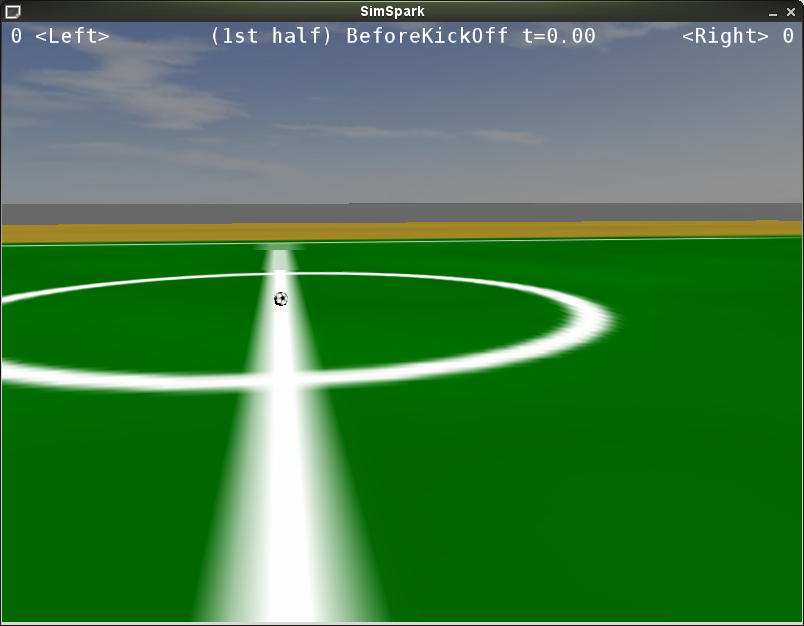
\includegraphics[width=0.8\textwidth]{fig/startup}
\caption{View of the soccer simulation after the simulator has just been started.}
\label{fig:startup}
\end{center}
\end{figure}

\begin{figure}[htbp]
\begin{center}
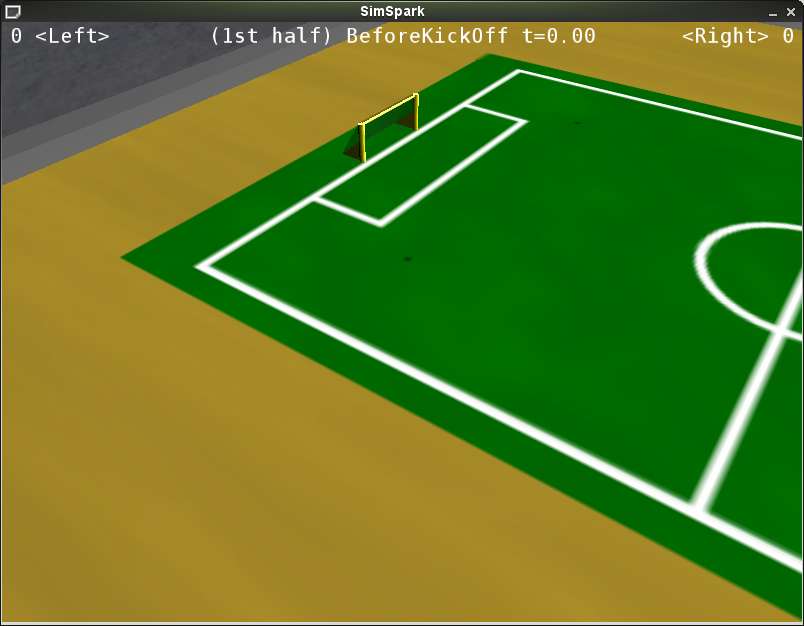
\includegraphics[width=0.8\textwidth]{fig/press3}
\caption{Change the view by pressing '3' on the keyboard.}
\label{fig:press3}
\end{center}
\end{figure}


\item{Connect an agent}

The next step is to connect one or more agents to the simulation. To
do this please change to a separate console window and type \texttt{rcssagent3d}.
This starts the example agent that is included with SimSpark. 

You should now see a humanoid robot appear on the field, as in figure
\ref{fig:agentconnect}. This default agent does nothing useful but waving his arms.

\begin{figure}[htbp]
\begin{center}
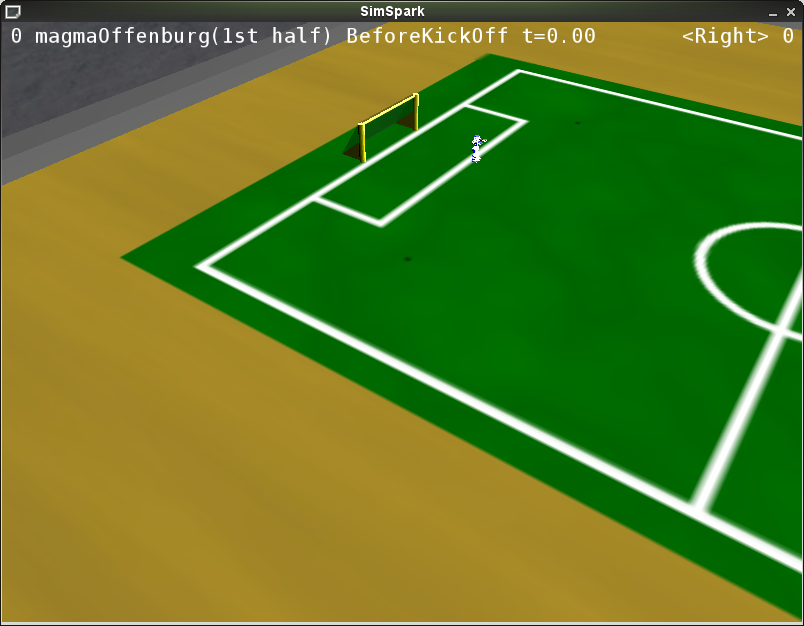
\includegraphics[width=0.8\textwidth]{fig/agentconnect}
\caption{An agent connected to the server.}
\label{fig:agentconnect}
\end{center}
\end{figure}

\begin{figure}[htbp]
\begin{center}
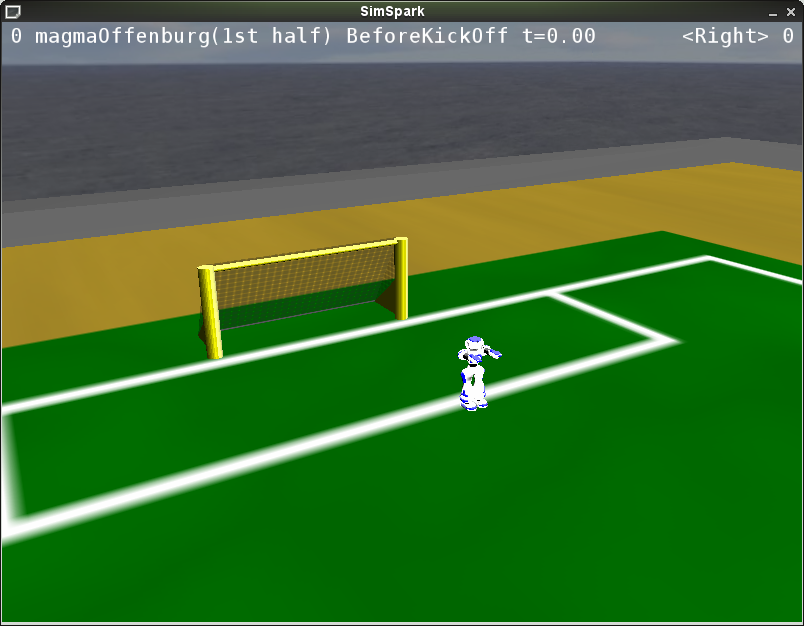
\includegraphics[width=0.8\textwidth]{fig/movearound}
\caption{Moving around on the field using the arrow keys, PgUp, PgDown, and the mouse (with left mouse button pressed).}
\label{fig:movearound}
\end{center}
\end{figure}


\item{Start the simulation}

The next step is to start the soccer game. To do this please change
back to the monitor window and press \texttt{'k'}. The simulation time
now start running and the game state changes to
\texttt{BeforeKickOff}, please compare to figure \ref{fig:presskickoff}.

\begin{figure}[htbp]
\begin{center}
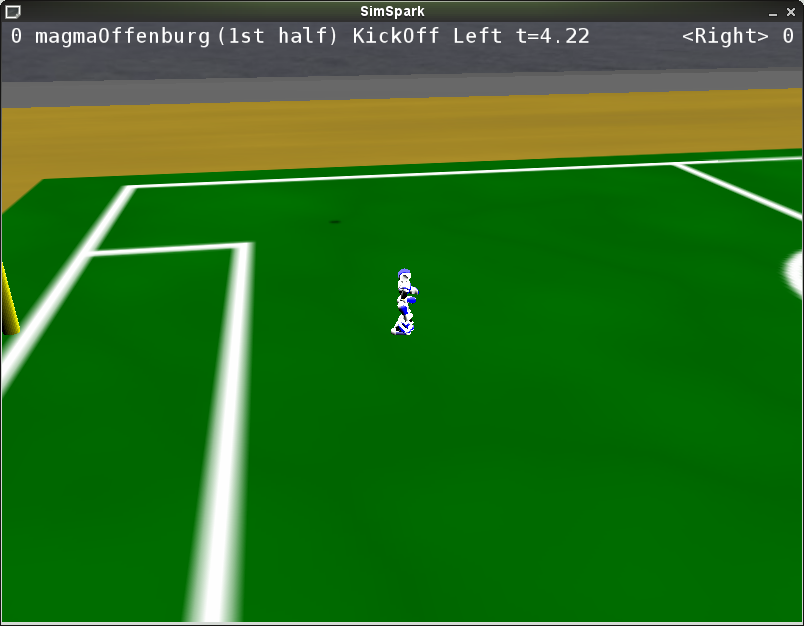
\includegraphics[width=0.8\textwidth]{fig/presskickoff}
\caption{Press 'k' to start the game. The play mode will switch to 'KickOff
Left' and the time will advance.}
\label{fig:presskickoff}
\end{center}
\end{figure}

\end{itemize}


%I think for the initial outline of the manual it's easier to just focus on either app/simpark app/rcssmonitor3d  or rsgedit.

%%% Local Variables: 
%%% mode: latex
%%% TeX-master: "user-manual"
%%% End: 
